%%% SemiCluster1.tex --- 
%% Version: $Id: SemiCluster1.tex,v 0.0 2012/05/09 09:17:01 tangboyun Exp$
%% Copyright : (c) 2012 Boyun Tang
%% License : BSD-style

\documentclass{standalone}
\usepackage{tikz}
\usetikzlibrary{mindmap,shadows,shapes,positioning,calc,}
\usepackage{graphicx}
\usepackage{times}
\usepackage{xcolor}

\begin{document}

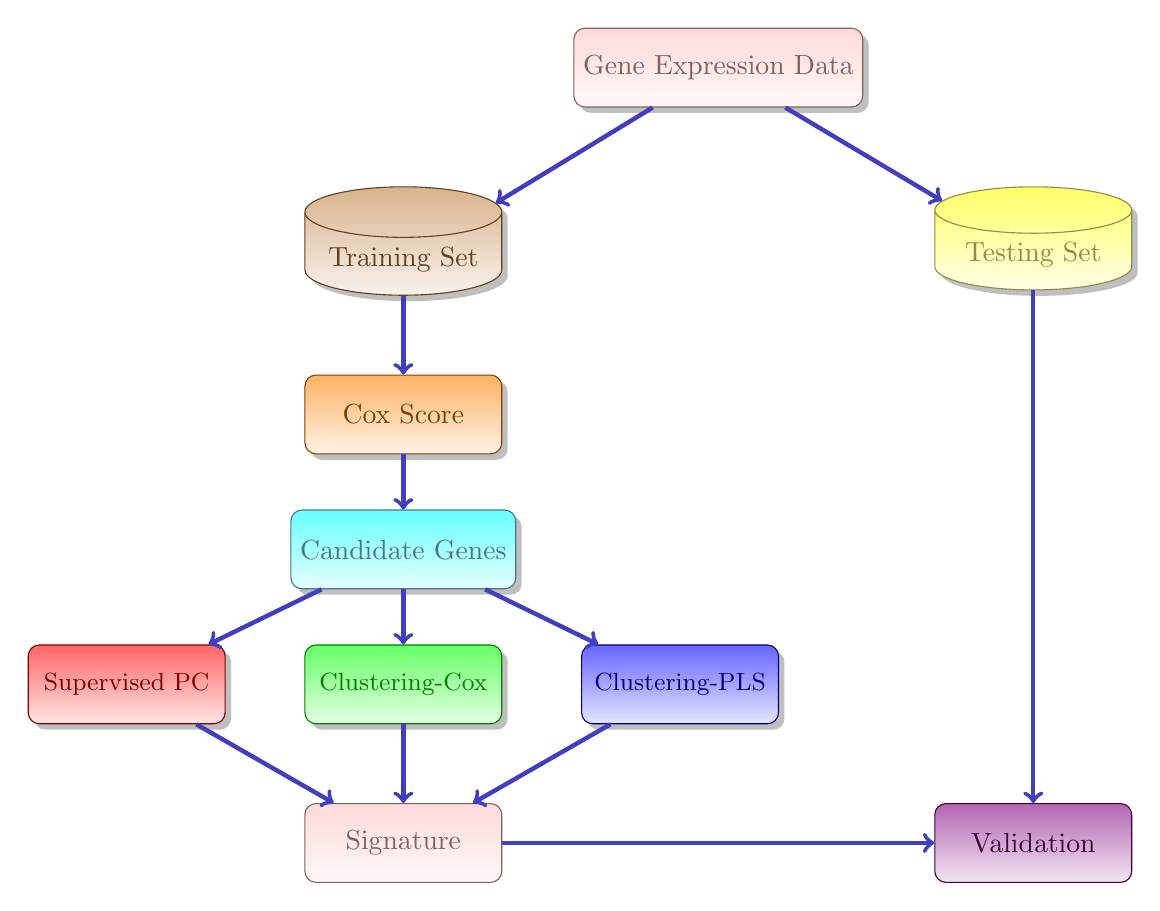
\begin{tikzpicture}[
  every node/.style={minimum width=2.5cm,minimum height=1cm,align=center,},%
  dr/.style={drop shadow},%
  e/.style={->,ultra thick,rounded corners,draw=blue!50!gray},%
  cl/.style={cylinder,aspect=.3,shape border rotate=90,},%
  re/.style={rounded corners,},%
  r/.style={top color= red!60,bottom color= red!10,draw=red!50!black,%
    text=red!50!black,},%
  g/.style={top color= green!60,bottom color= green!10,draw=green!50!black,%
    text=green!50!black,},%
  b/.style={top color= blue!60,bottom color= blue!10,draw=blue!50!black,%
    text=blue!50!black,},%
  br/.style={top color= brown!60,bottom color= brown!10,draw=brown!50!black,%
    text=brown!50!black,},%
  v/.style={top color= violet!60,bottom color= violet!10,draw=violet!50!black,%
    text=violet!50!black,},%
  o/.style={top color= orange!60,bottom color= orange!10,draw=orange!50!black,%
    text=orange!50!black,},%
  ye/.style={top color= yellow!60,bottom color= yellow!10,draw=yellow!50!black,%
    text=yellow!50!black,},%
  p/.style={top color= pink!60,bottom color= pink!10,draw=pink!50!black,%
    text=pink!50!black,},%
  c/.style={top color= cyan!60,bottom color= cyan!10,draw=cyan!50!black,%
    text=cyan!50!black,},%
  a/.style={single arrow,draw,bottom color=red,top color=white,shape border uses incircle,
    shape border rotate=-90,minimum height=.85cm,minimum width=0.1cm,scale=.5}
  ]

  \node (sample) [re,p,dr%
  ] {Gene Expression Data};

  \node (train) [cl,below=of sample,xshift=-4cm,br,dr%
  ] {Training Set};

  \node (test) [cl,below=of sample,xshift=4cm,ye,dr%
  ] {Testing Set};
  
  \node (tt) [below=of train,re,o,dr] {Cox Score};

  \node (can) [below=of tt,re,c,yshift=0.3cm,dr] {Candidate Genes};

  \node (cox) [dr,below=of can,g,
  font=\small,yshift=0.3cm,re] {Clustering-Cox};
  \node (pc) [dr,left=of cox,r,font=\small,re] {Supervised PC};
  \node (pls) [dr,right=of cox,b,font=\small,re] {Clustering-PLS};
  \node (sig) [below=of cox,re,p] {Signature};

  \path let \p1 = (sig.center), \p2=(test.center) in node (valid) [v,re] at (\x2,\y1) {Validation}; 
  \draw [e] (train) -- (tt);
  \draw [e] (tt) -- (can);
  \draw [e] (can) -- (pc);
  \draw [e] (can) -- (pls);
  \draw [e] (can) -- (cox);
  \draw [e] (cox) -- (sig);
  \draw [e] (pc) -- (sig);
  \draw [e] (pls) -- (sig);
  \draw [e] (test) -- (valid);
  \draw [e] (sig) -- (valid);
  \draw [e] (sample) -- (train);
  \draw [e] (sample) -- (test);
\end{tikzpicture}
\end{document}


%%% Local Variables: 
%%% TeX-master: t
%%% End: 
